\documentclass[border={0pt 0pt 0pt 0pt},convert={density=300,outext=.png}]{standalone}

\usepackage{tikz}
\usepackage{pgf}
\usepackage{subcaption}
% \usepackage[margin=0.5pt]{geometry}
\usetikzlibrary{calc}   % coordinate calculation

\newcommand{\defstuff} {
  \def \step {1}
  \def \cc {\step/2}  % center of cell
  \coordinate (offset) at ($(\cc,\cc)$);
}

\newcommand{\drawgrid}[1] {
  \draw[step=\step, color=gray] (0,0) grid ($#1$); % draw the grid, base at #1
}

\newcommand{\drawrobots}[1] {
    \foreach \coord in #1 {
      \coordinate[at=\coord, name=A];
      \draw ($(A) + (offset)$) circle ({\cc*0.8});
    }
}

\newcommand{\drawarrows}[1] {
    \foreach \a/\b in #1 {
      \coordinate[at=\a, name=A];
      \coordinate[at=\b, name=B];
      \draw[->, color=darkgray] ($(A) + (offset)$) -- ($(B) + (offset)$);
    }
}

\newcommand{\spacee}[3] {
  \begin{tikzpicture}[thick, scale=0.6]
    \defstuff
    \drawgrid{#1}
    \drawrobots{#2}
    \drawarrows{#3}
  \end{tikzpicture}
}


\begin{document}

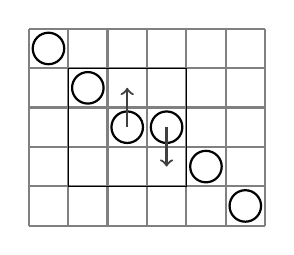
\begin{tikzpicture}[thick, scale=0.5]
\defstuff
\drawgrid{(6,5)}
\fillrobots{{(2,2)}}{red}
\fillrobots{{(3,2)}}{blue}
\drawrobots{{(0,4),(1,3),(2,2),(3,2),(4,1),(5,0)}}
\drawarrows{{{(2,2)/(2,3)},{(3,2)/(3,1)}}}
\draw[thin] (1,1) -- (4,1) -- (4,4) -- (1,4) -- (1,1);
\end{tikzpicture}


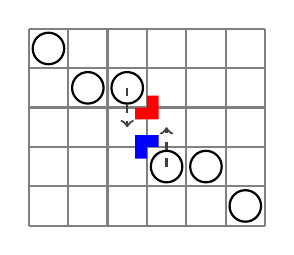
\begin{tikzpicture}[thick, scale=0.5]
\defstuff
\drawgrid{(6,5)}
\fillrobots{{(2,3)}}{red}
\fillrobots{{(3,1)}}{blue}
\drawrobots{{(0,4),(1,3),(2,3),(3,1),(4,1),(5,0)}}
% \drawarrows{{{(2,2)/(2,3)},{(3,2)/(3,1)}}}
\draw[->,color=darkgray,dashed] (2.5,3.5) -- (2.5,2.5);
\draw[->,color=darkgray,dashed] (3.5,1.5) -- (3.5,2.5);
\fill[red]  (3,3) -- (3,3.3) -- (3.3,3.3) -- (3.3,2.7) -- (2.7,2.7) -- (2.7,3) -- (3,3);
\fill[blue] (3,2) -- (3.3,2) -- (3.3,2.3) -- (2.7,2.3) -- (2.7,1.7) -- (3,1.7) -- (3,2);
\end{tikzpicture}

\end{document}
